\documentclass[%
 reprint,
 amsmath,amssymb
 aps,
]{revtex4-2}

\usepackage{float}

\usepackage{graphicx}% Include figure files
\usepackage{dcolumn}% Align table columns on decimal point
\usepackage{bm}% bold math
\usepackage{physics}
\setlength{\parskip}{\baselineskip}%
\usepackage{siunitx}
\usepackage[inline]{asymptote}
\usepackage{multirow}
\usepackage{tikz}
\usepackage{pgfplots, pgfplotstable}
% \def\bibsection{\section*{\refname}} 
\usepackage{hyperref}
% \usepackage{natbib}
% \bibliographystyle{unsrtnat}

\pgfplotsset{compat=1.3}
\begin{document}

% \preprint{APS}

\title{Verifying Length and Mass Dependance of the Period of a Homemade Pendulum}% Force line breaks with \\

\author{QiLin Xue}

\date{\today}% It is always \today, today,
             %  but any date may be explicitly specified

\begin{abstract}
This experiment analyzed the effects of changing the length and mass on the period of a home-made pendulum. The data for the period was obtained by releasing the pendulum from a small angle and slowly changing its length by connecting it to a pulley system. The mass dependance was measured by manually timing the pendulum with a stopwatch and changing the mass by manually pouring out water. In general, both agreed with theory, providing the correct coefficients. However, more work needs to be done to measure and quantify other effects such as a changing center of mass, a nonzero moment of inertia, and air resistance for complete model validation.
\end{abstract}

%\keywords{Suggested keywords}%Use showkeys class option if keyword
                              %display desired
\maketitle

%\tableofcontents
\section{Introduction}
Previous experiments have established methods to analyze the motion of a pendulum using a motion tracker and applying computational techniques. These methods were applied to determine the quality factor $Q$ of a homemade pendulum, as well as verifying the amplitude dependance on the period. To complete the validation, I aim to determine how mass and length affects the period and compare it with the theoretical predictions.

While in previous experiments, I have modeled the water bottle to be a point mass, which is valid within experimental error, this may not be as accurate when the string length decreases. For a compound pendulum, the period is given by:
\begin{equation}
    T = 2\pi\sqrt{\frac{I}{mg\ell_\text{cm}}}
    \label{eq:}
\end{equation}
If the moment of inertia of the water bottle around the center of mass is $I_\text{cm}=\beta m d^2$ where $d$ is the length of the water bottle, then by the parallel axis theorem, the period can be written as:
\begin{equation}
    T = 2\pi\sqrt{\frac{\beta d^2 + \ell_\text{cm}^2}{g\ell_\text{cm}}}
    \label{eq:proper}
\end{equation}
A nicer form to work with would be the lowest order approximation
\begin{equation}
    T = 2\pi\sqrt{\frac{\ell_\text{cm}}{g}}\left(1+\frac{\beta d^2}{2\ell_\text{cm}^2}\right)
    \label{eq:low order}
\end{equation}
Since mass does not appear in this equation, I would not expect the period to be affected by increasing the mass if all other quantities are the same. Since the mass is changed by removing or adding water from the bottle, the center of mass is able to change. I can approximate the bottle as a rectangular prism with a height of $13.2 \pm 0.1 \si{\centi\meter}$ and a base consisted of a square with side lengths $5.0 \pm 0.1 \si{\centi\meter}$ such that the total volume is around $330\si{\milli\meter}$. An empty bottle weighs $29 \pm 0.5 \si{\gram}$ and assuming the mass distribution is constant, the center of mass of the bottle when the water is at a height $h$ is given by:
\begin{equation}
    d_\text{cm} = \frac{\left(\rho(5.0)^2h\right)\frac{h}{2} + 29\left(\frac{13.2}{2}\right)}{29+\left(\rho(5.0)^2h\right)}
    \label{eq:}
\end{equation}
which reaches a maximum of $d_\text{cm,max}=6.6\si{\centi\meter}$ and a minimum of $d_\text{cm,min}=2.9\si{\centi\meter}$ such that the effective uncertainty of the center of mass can be seen as $\delta \ell_\text{cm}=6.6-2.9 = 0.037\si{\meter}$. The relative uncertainty in the period is given by:
\begin{equation}
    \frac{\delta T}{T} \approx \frac{\delta \ell_\text{cm}}{2\ell_\text{cm}} \implies \delta T = \frac{\delta \ell}{2\sqrt{g\ell_\text{cm}}}
    \label{eq:}
\end{equation}
If approximately a two meter long string is used, then the uncertainty in the period is:
\begin{equation}
    \delta T \approx 0.004\si{\second}
    \label{eq:}
\end{equation}
My reaction speed to a predictable visual event is $0.04 \pm 0.02\si{\second}$, which was obtained by attempting to stop the stopwatch on the iPhone ``clock app'' every time the second hand crosses the five second mark. If ten oscillations are used to determine the period, then the uncertainty in the period measurement will be on the same order of magnitude as $\delta T$. Therefore, even though the center of mass of the pendulum will be changing, it is very likely no trend will be seen.
\section{Method and Modifications}
To reduce potential sources of error, the \textit{Tracker} program was used again for the first part of this experiment.. In order to make it easier to change length, the pendulum was attached to a pulley system as shown in figure \ref{fig:cool}. As the bottle swings, the other end of the pulley was pulled down such that the length changes roughly adiabatically (slowly, no external torques are applied). A GoPro camera was used to record at 120 fps, such that the time uncertainty for a single oscillation is $\delta t = 0.004 \si{\second}$, which is equal to the uncertainty if I had manually timed it for ten oscillations. As a result, by slowly and continuously changing the length, I was able to get period measurements for $200$ different lengths to a good precision. These measurements were then grouped together into $40$ data points by taking the average of consecutive five trials.
\begin{figure}[!h]
    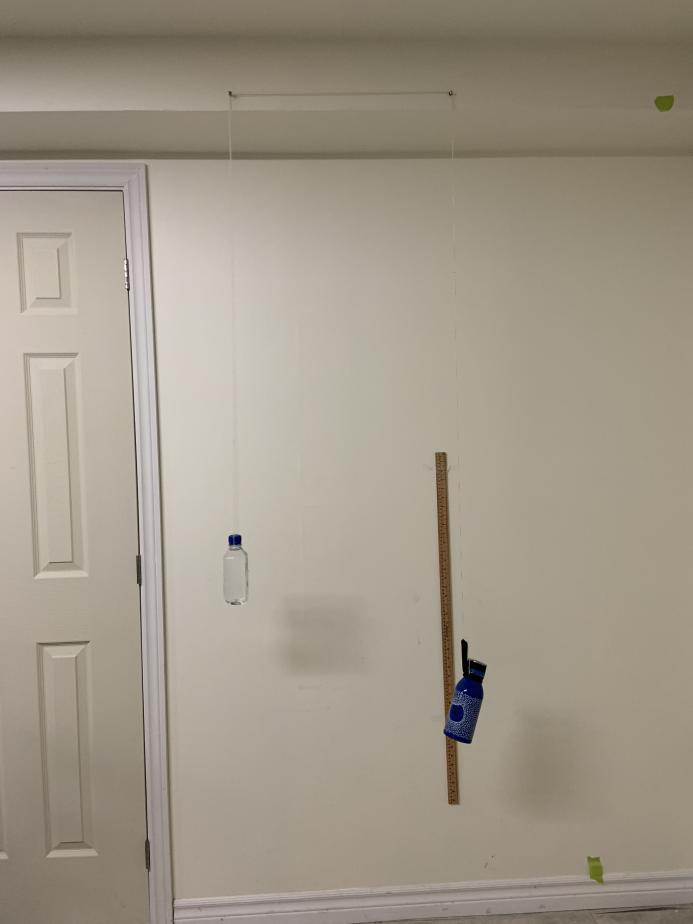
\includegraphics[width=\linewidth]{Figures/cool_beans.jpg}

    \caption{The modified pendulum setup. Another mass is tied to the right end, which allowed it to easily change the length of the swinging pendulum (left). A ruler is taped in the background for calibration purposes.}
    \label{fig:cool}
\end{figure}
Unfortunately, there was no easy way to change the mass so the oscillations were recorded manually. The mass of the pendulum was changed by dumping out small portions of the water after each trial, then using the pulley system to lower the pendulum onto a scale to take the mass measurement while making sure the tension in the string is zero. A mark was made on the string to ensure that the length of the string does not change between trials.

All trials for both parts were run with an initial angle less than $11.1^\circ$, which was determined to be the threshold at which the amplitude dependance of the period becomes unimportant.
\section{Results}
\subsection{Length Dependance}
I will linearize the data in two different ways: first by plotting the square of the period $T^2$ against the length of the string $\ell$ as seen in figure \ref{fig:linear-1}. This is done in order to determine relevant coefficients and determine the center of mass. Then I will plot $\log(\ell_\text{cm}+\Delta L)$ against $\log(T)$ to determine that the relationship is a square root model, which is shown in figure \ref{fig:log-2}.
\begin{figure}[!h]
    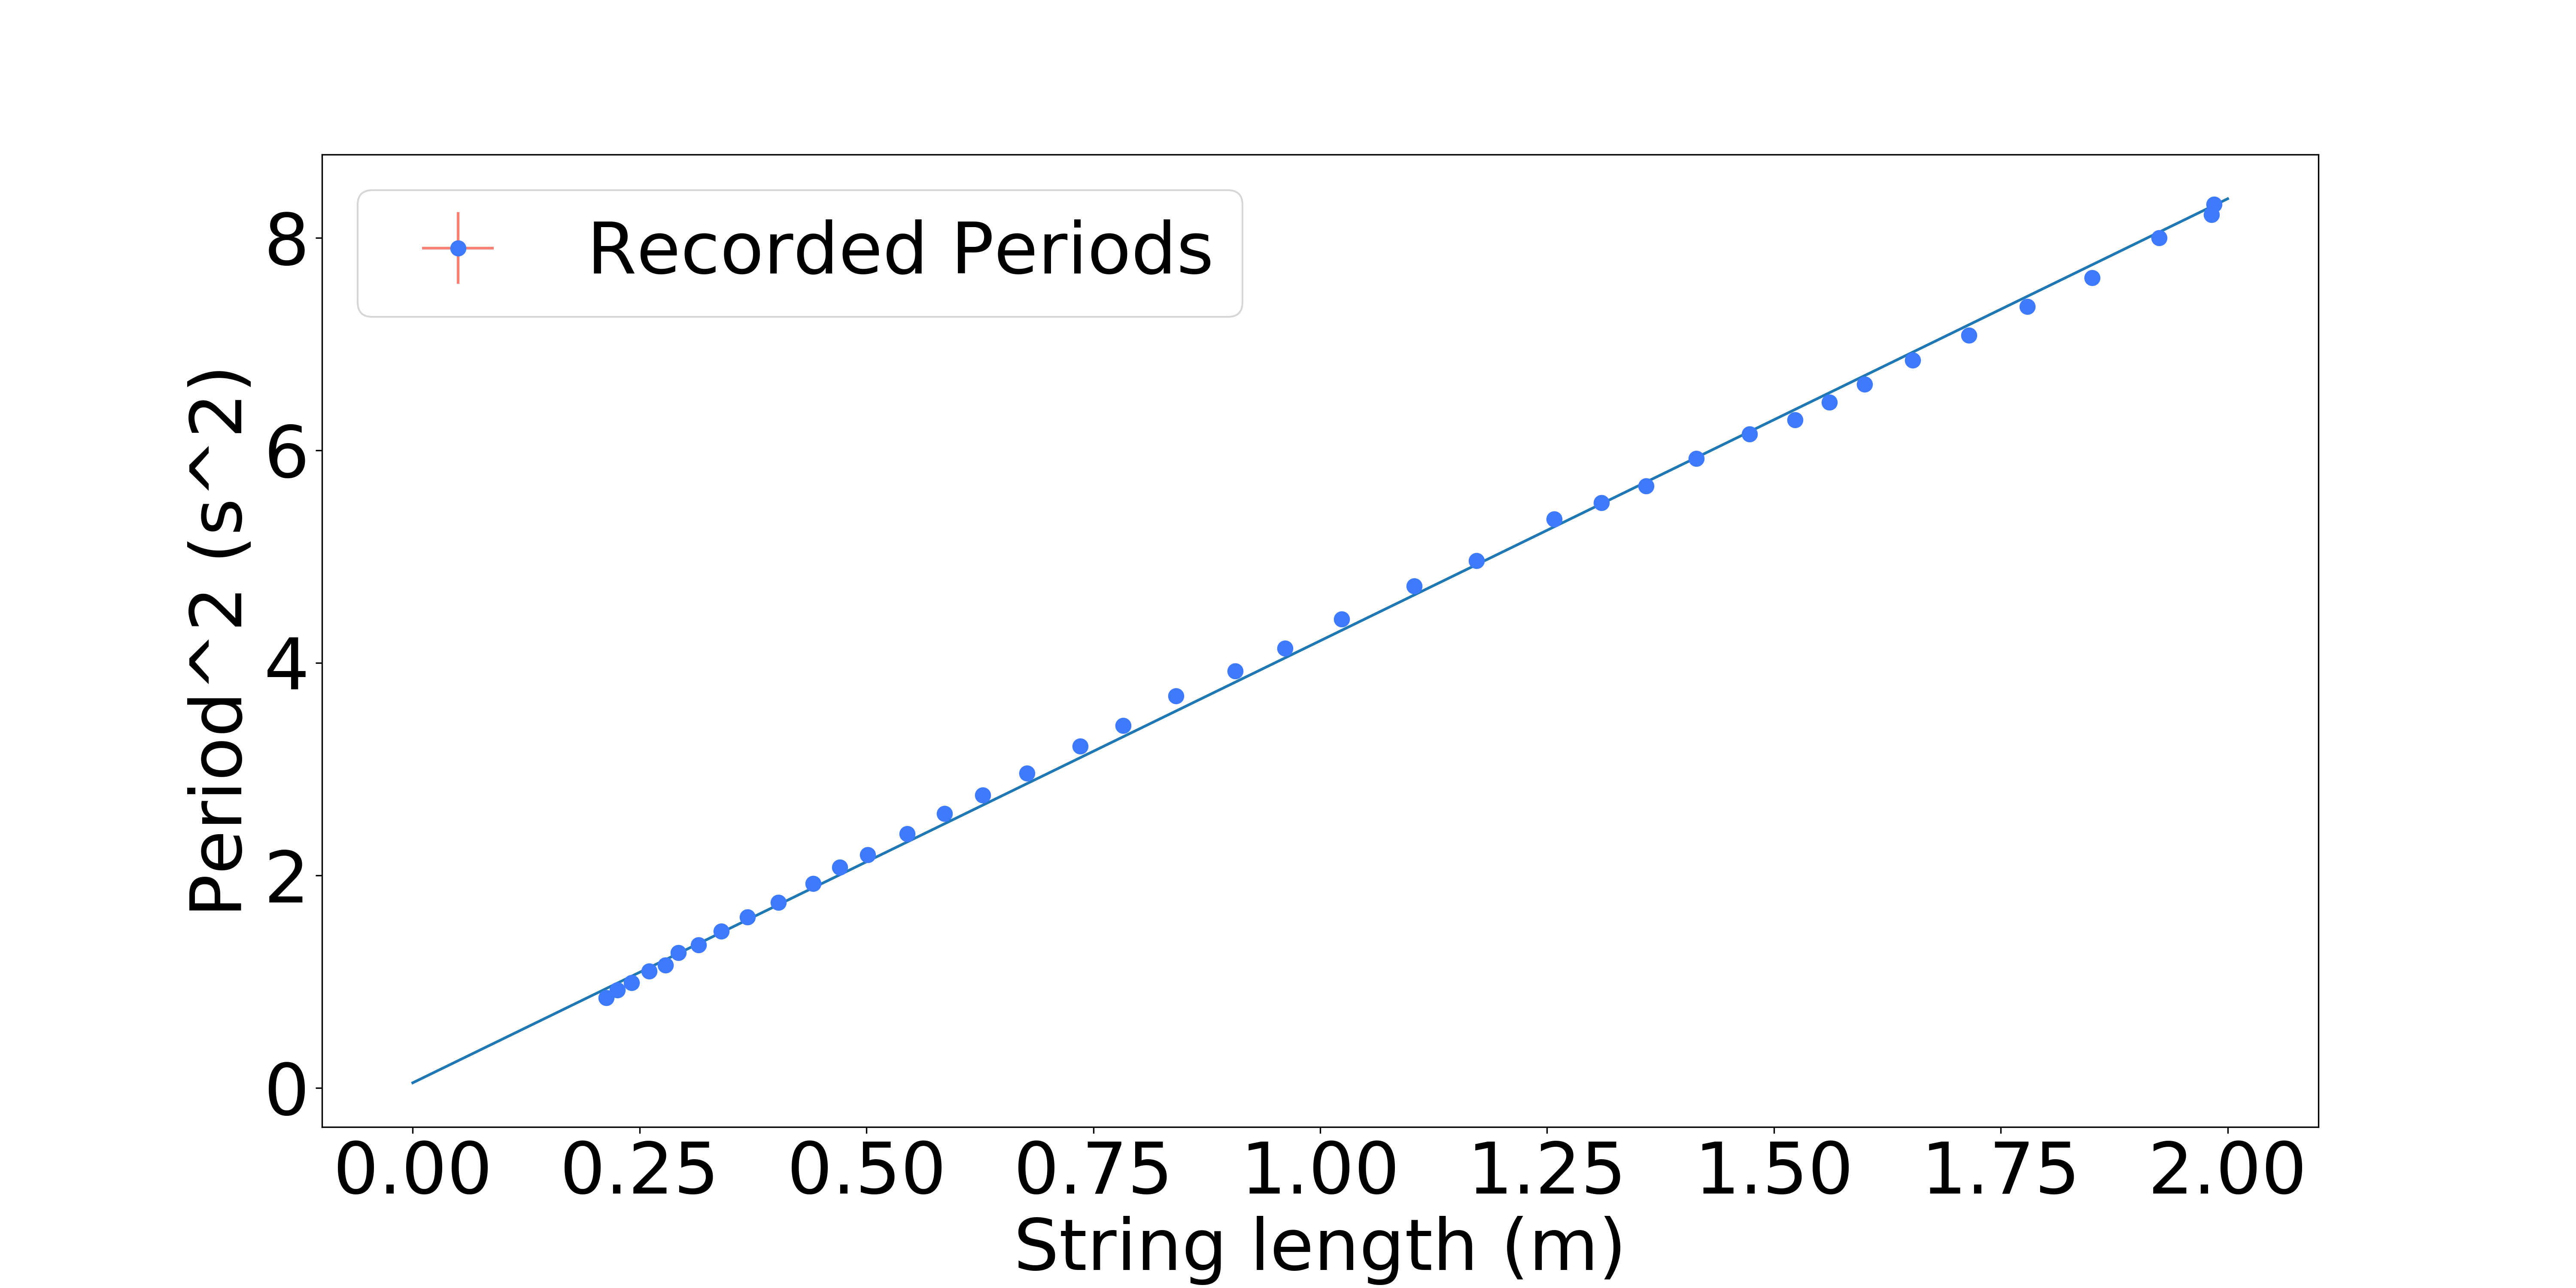
\includegraphics[width=\linewidth]{Figures/linear_1.png}
    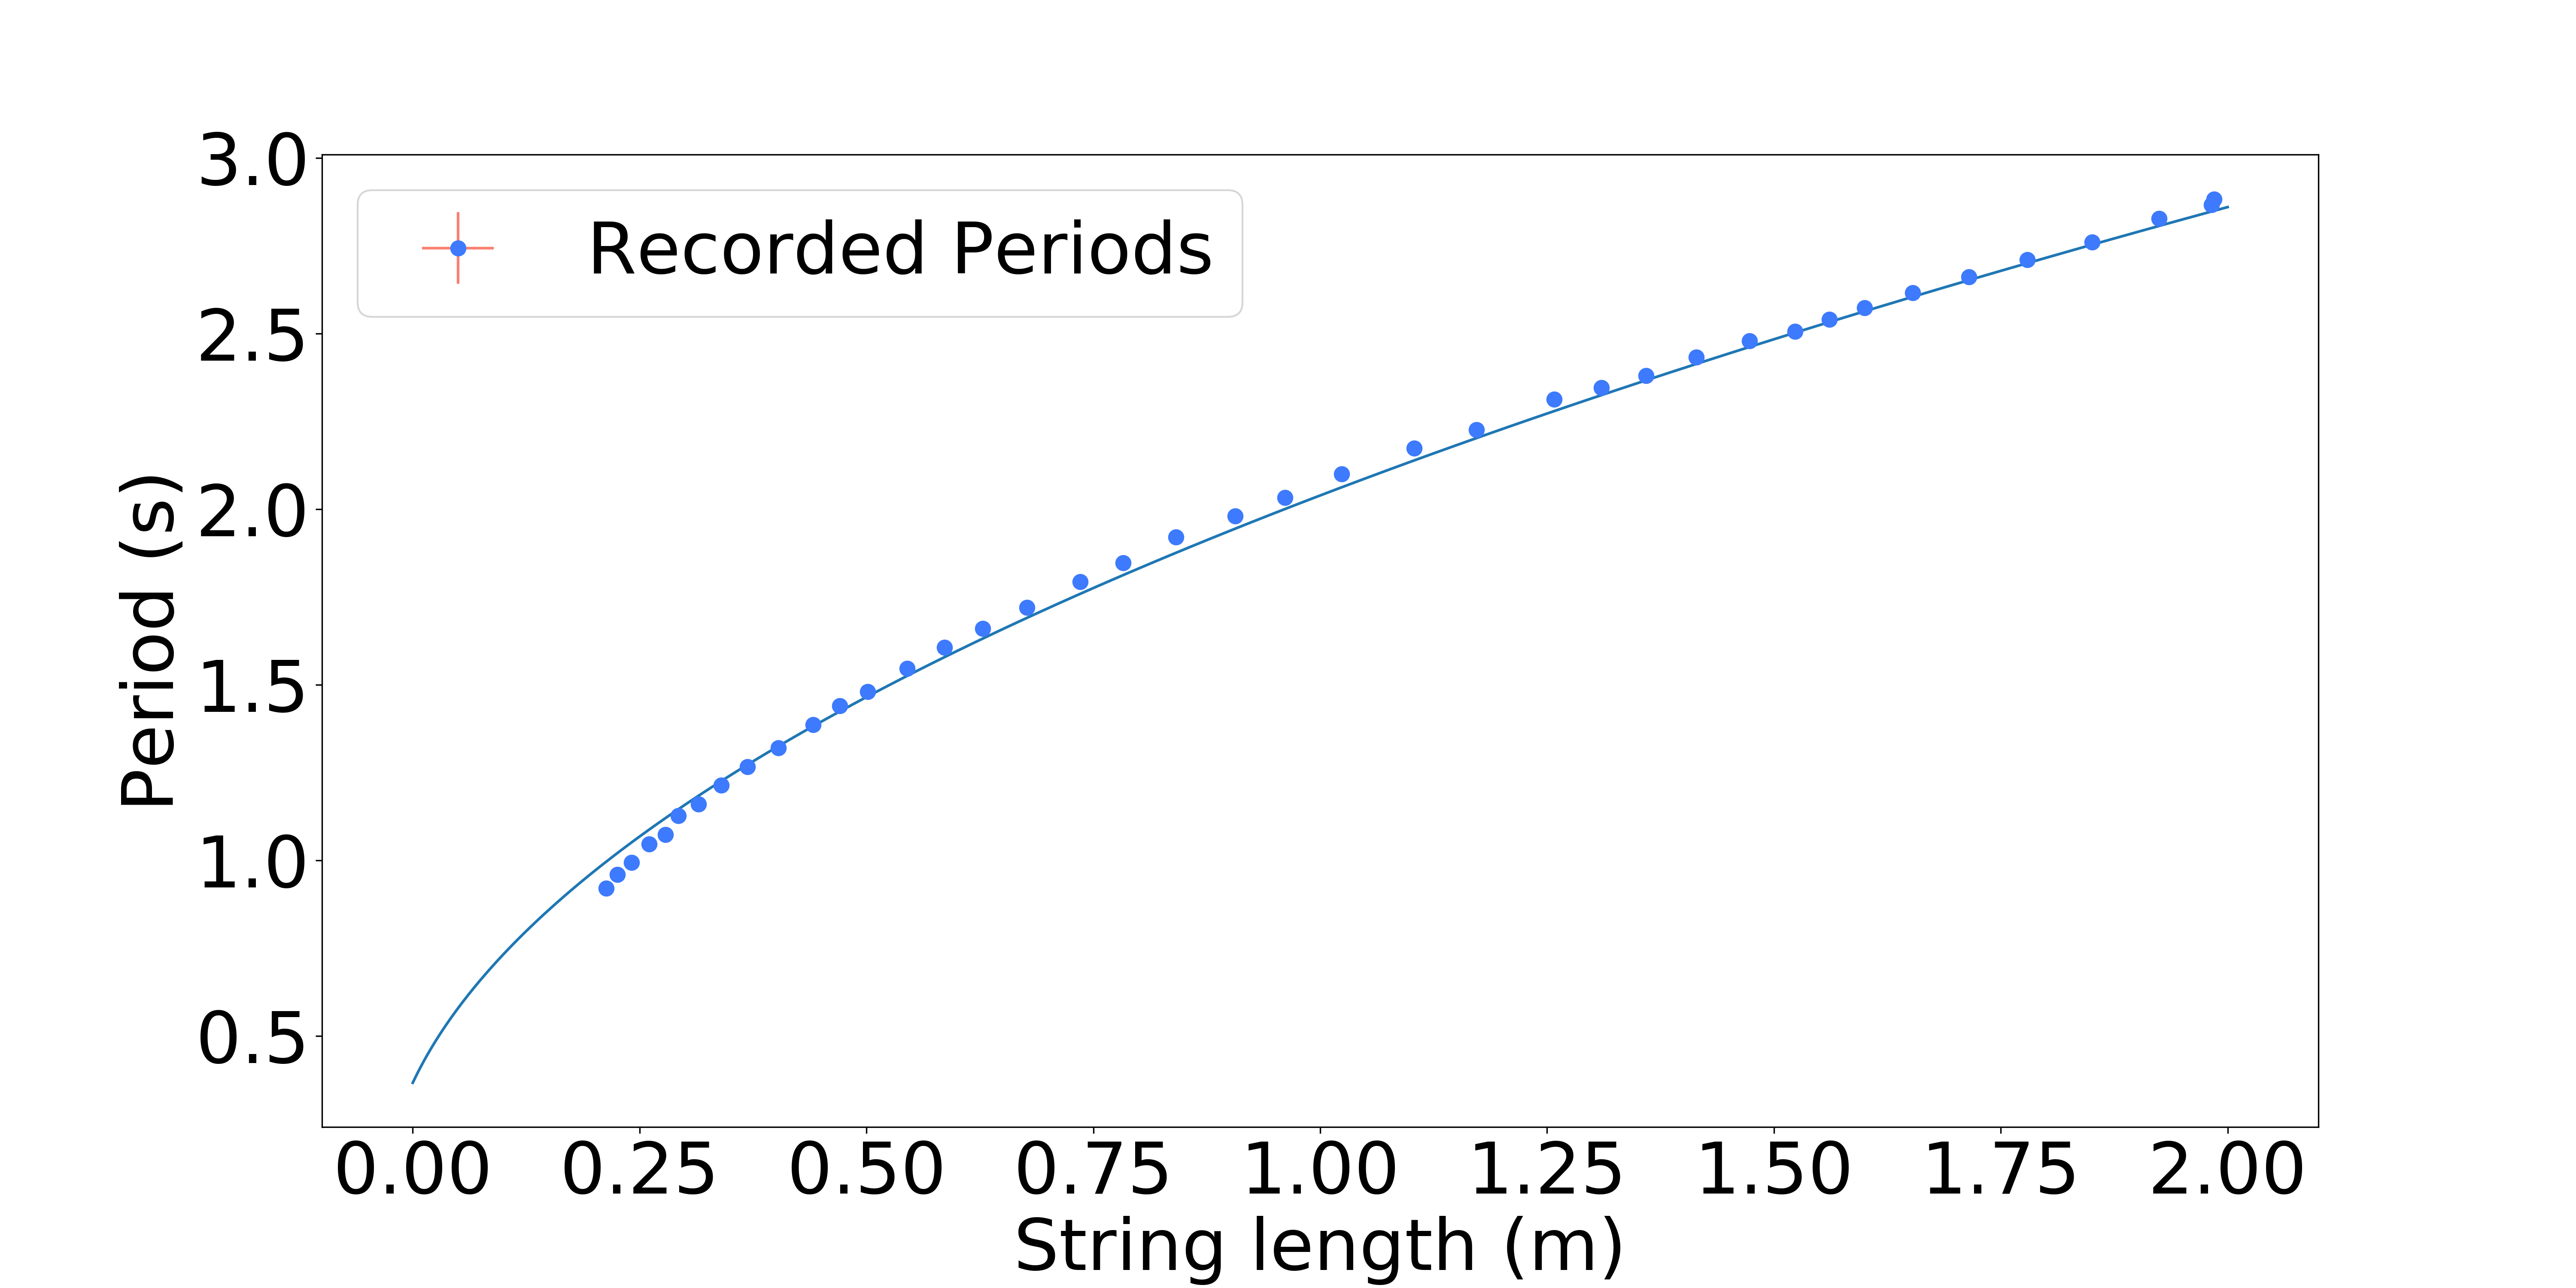
\includegraphics[width=\linewidth]{Figures/normal_1.png}

    \caption{Above: A plot of the square of the period against the length of the string. Below: A plot of only the period against the length of the rope. Note that the fitted curve overestimates the period for short string lengths.}
    \label{fig:linear-1}
\end{figure}
For the linearization, the slope $m$ and intercept $b$ are given by:
\begin{align}
    m &= 4.16 \pm 0.02 \si{\second\squared\per\meter} \\ 
    b &= 0.05 \pm 0.02 \si{\second\squared}
\end{align}
However, since the formula $T = 2\pi\sqrt{\frac{\ell_\text{cm}}{g}}$ is not accurate when the string length is comparable in size to the length of the water bottle, the two curves plotted in figure \ref{fig:linear-1} are not representative of the true curve. Instead, it may be better to only plot the half of the data which use a larger string length, as shown in figure \ref{fig:plot-2}
\begin{figure}[!h]
    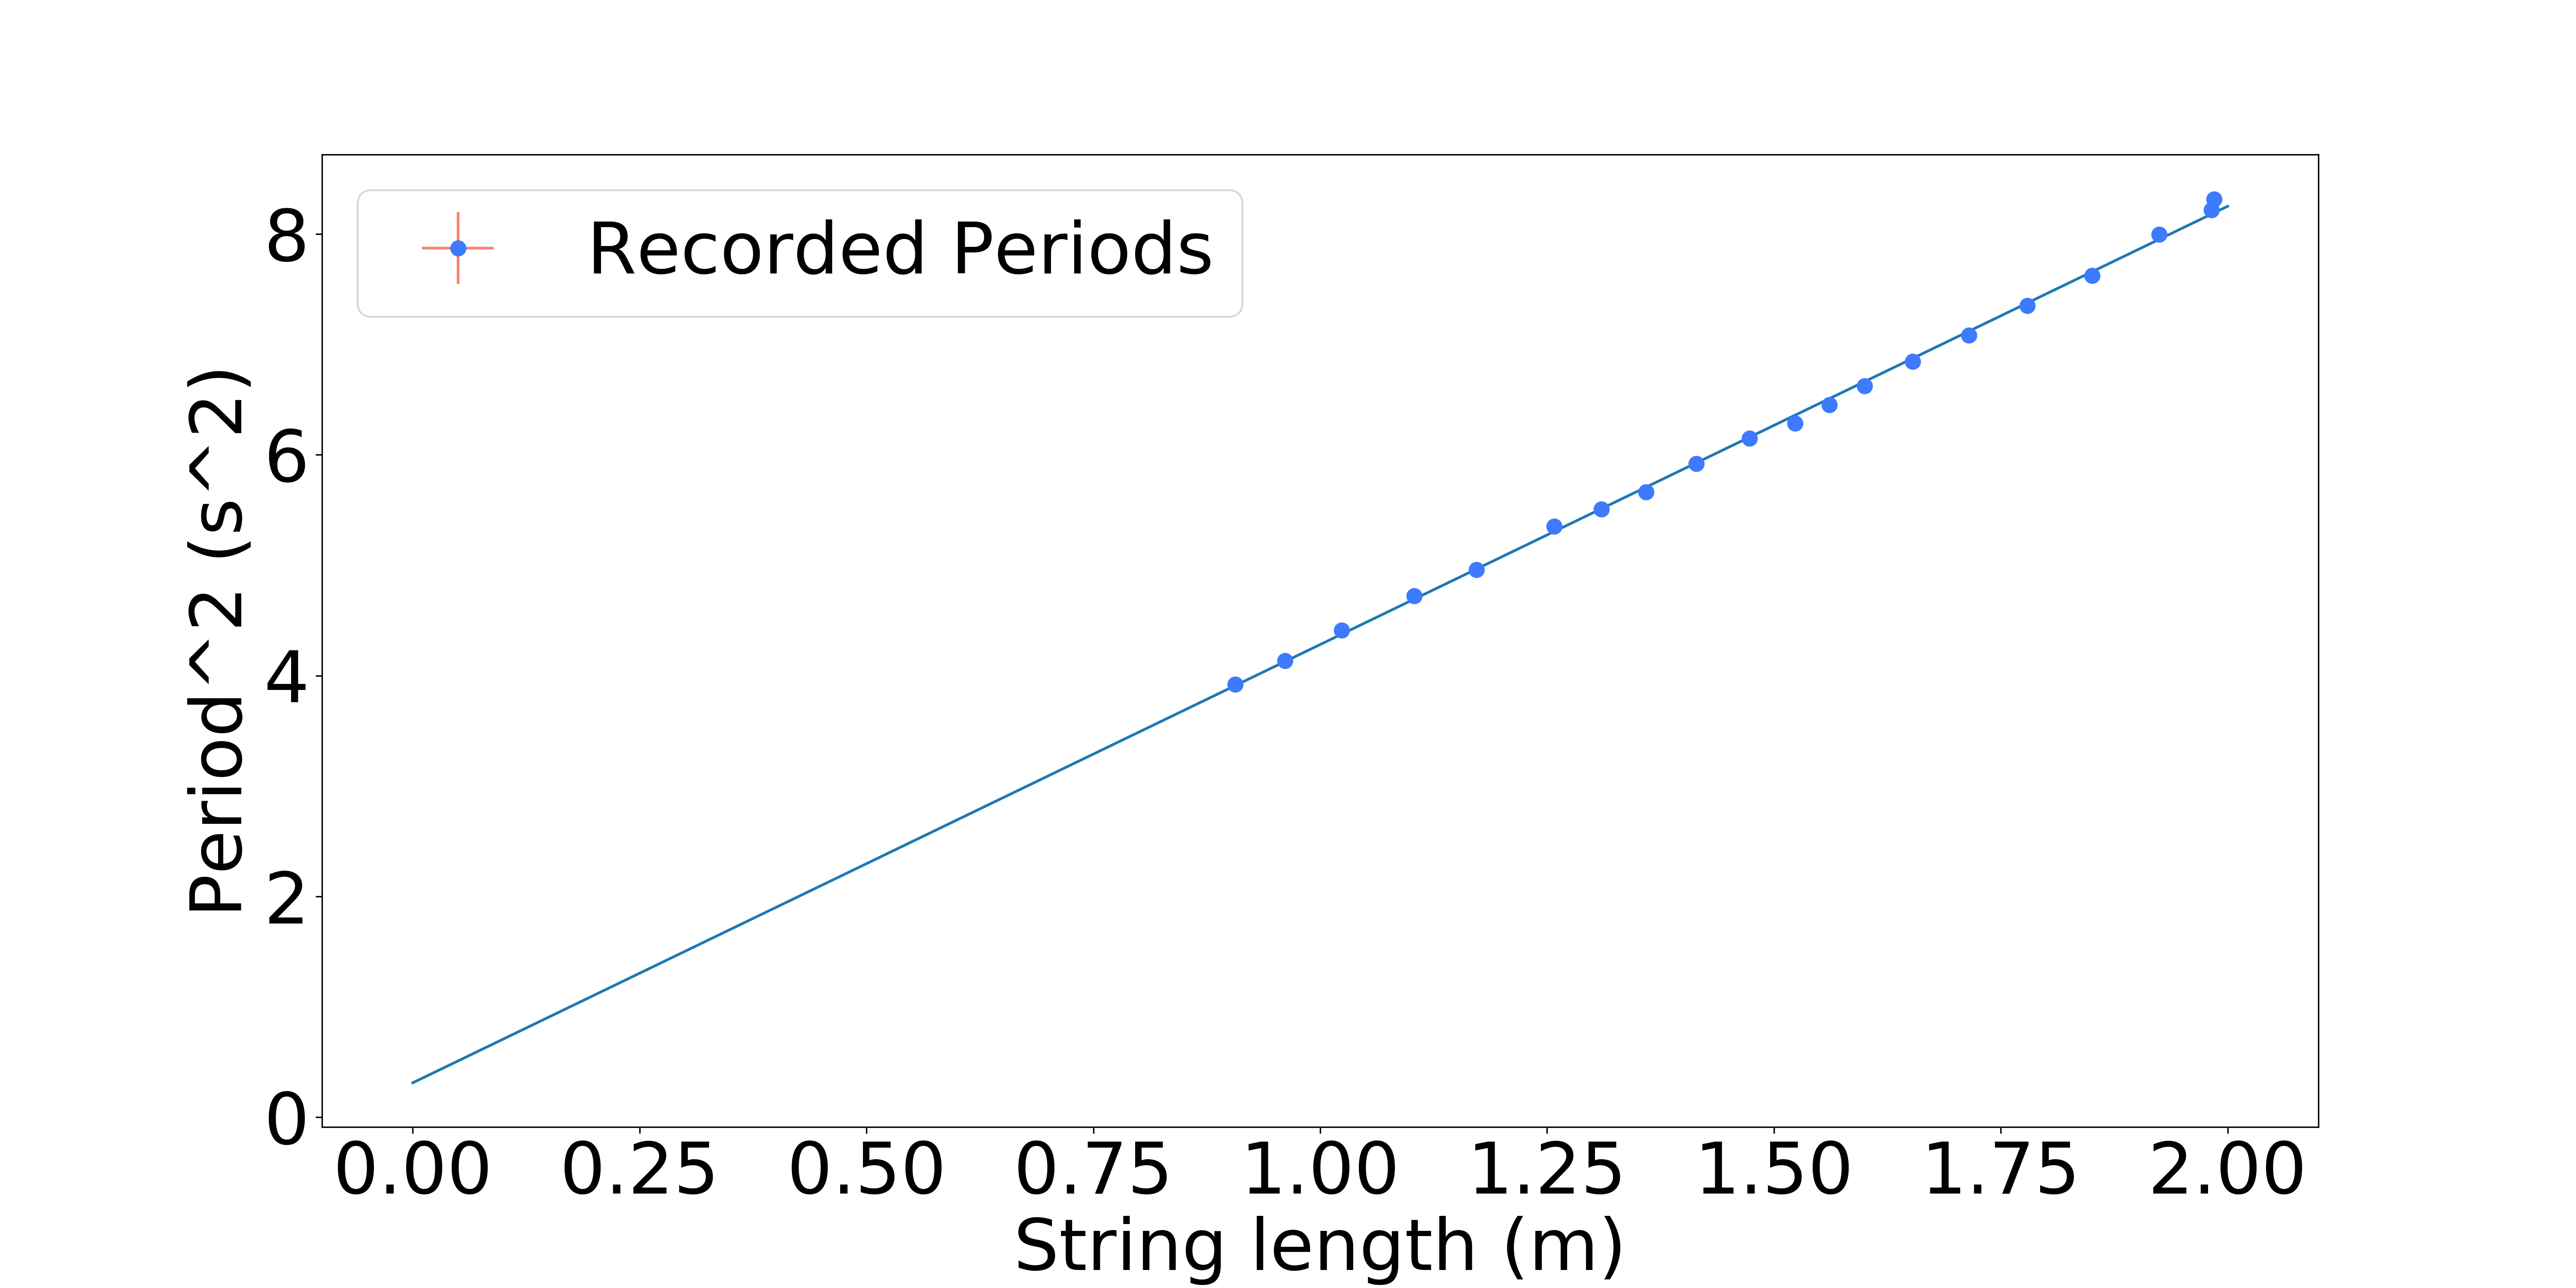
\includegraphics[width=\linewidth]{Figures/linear_2.png}
    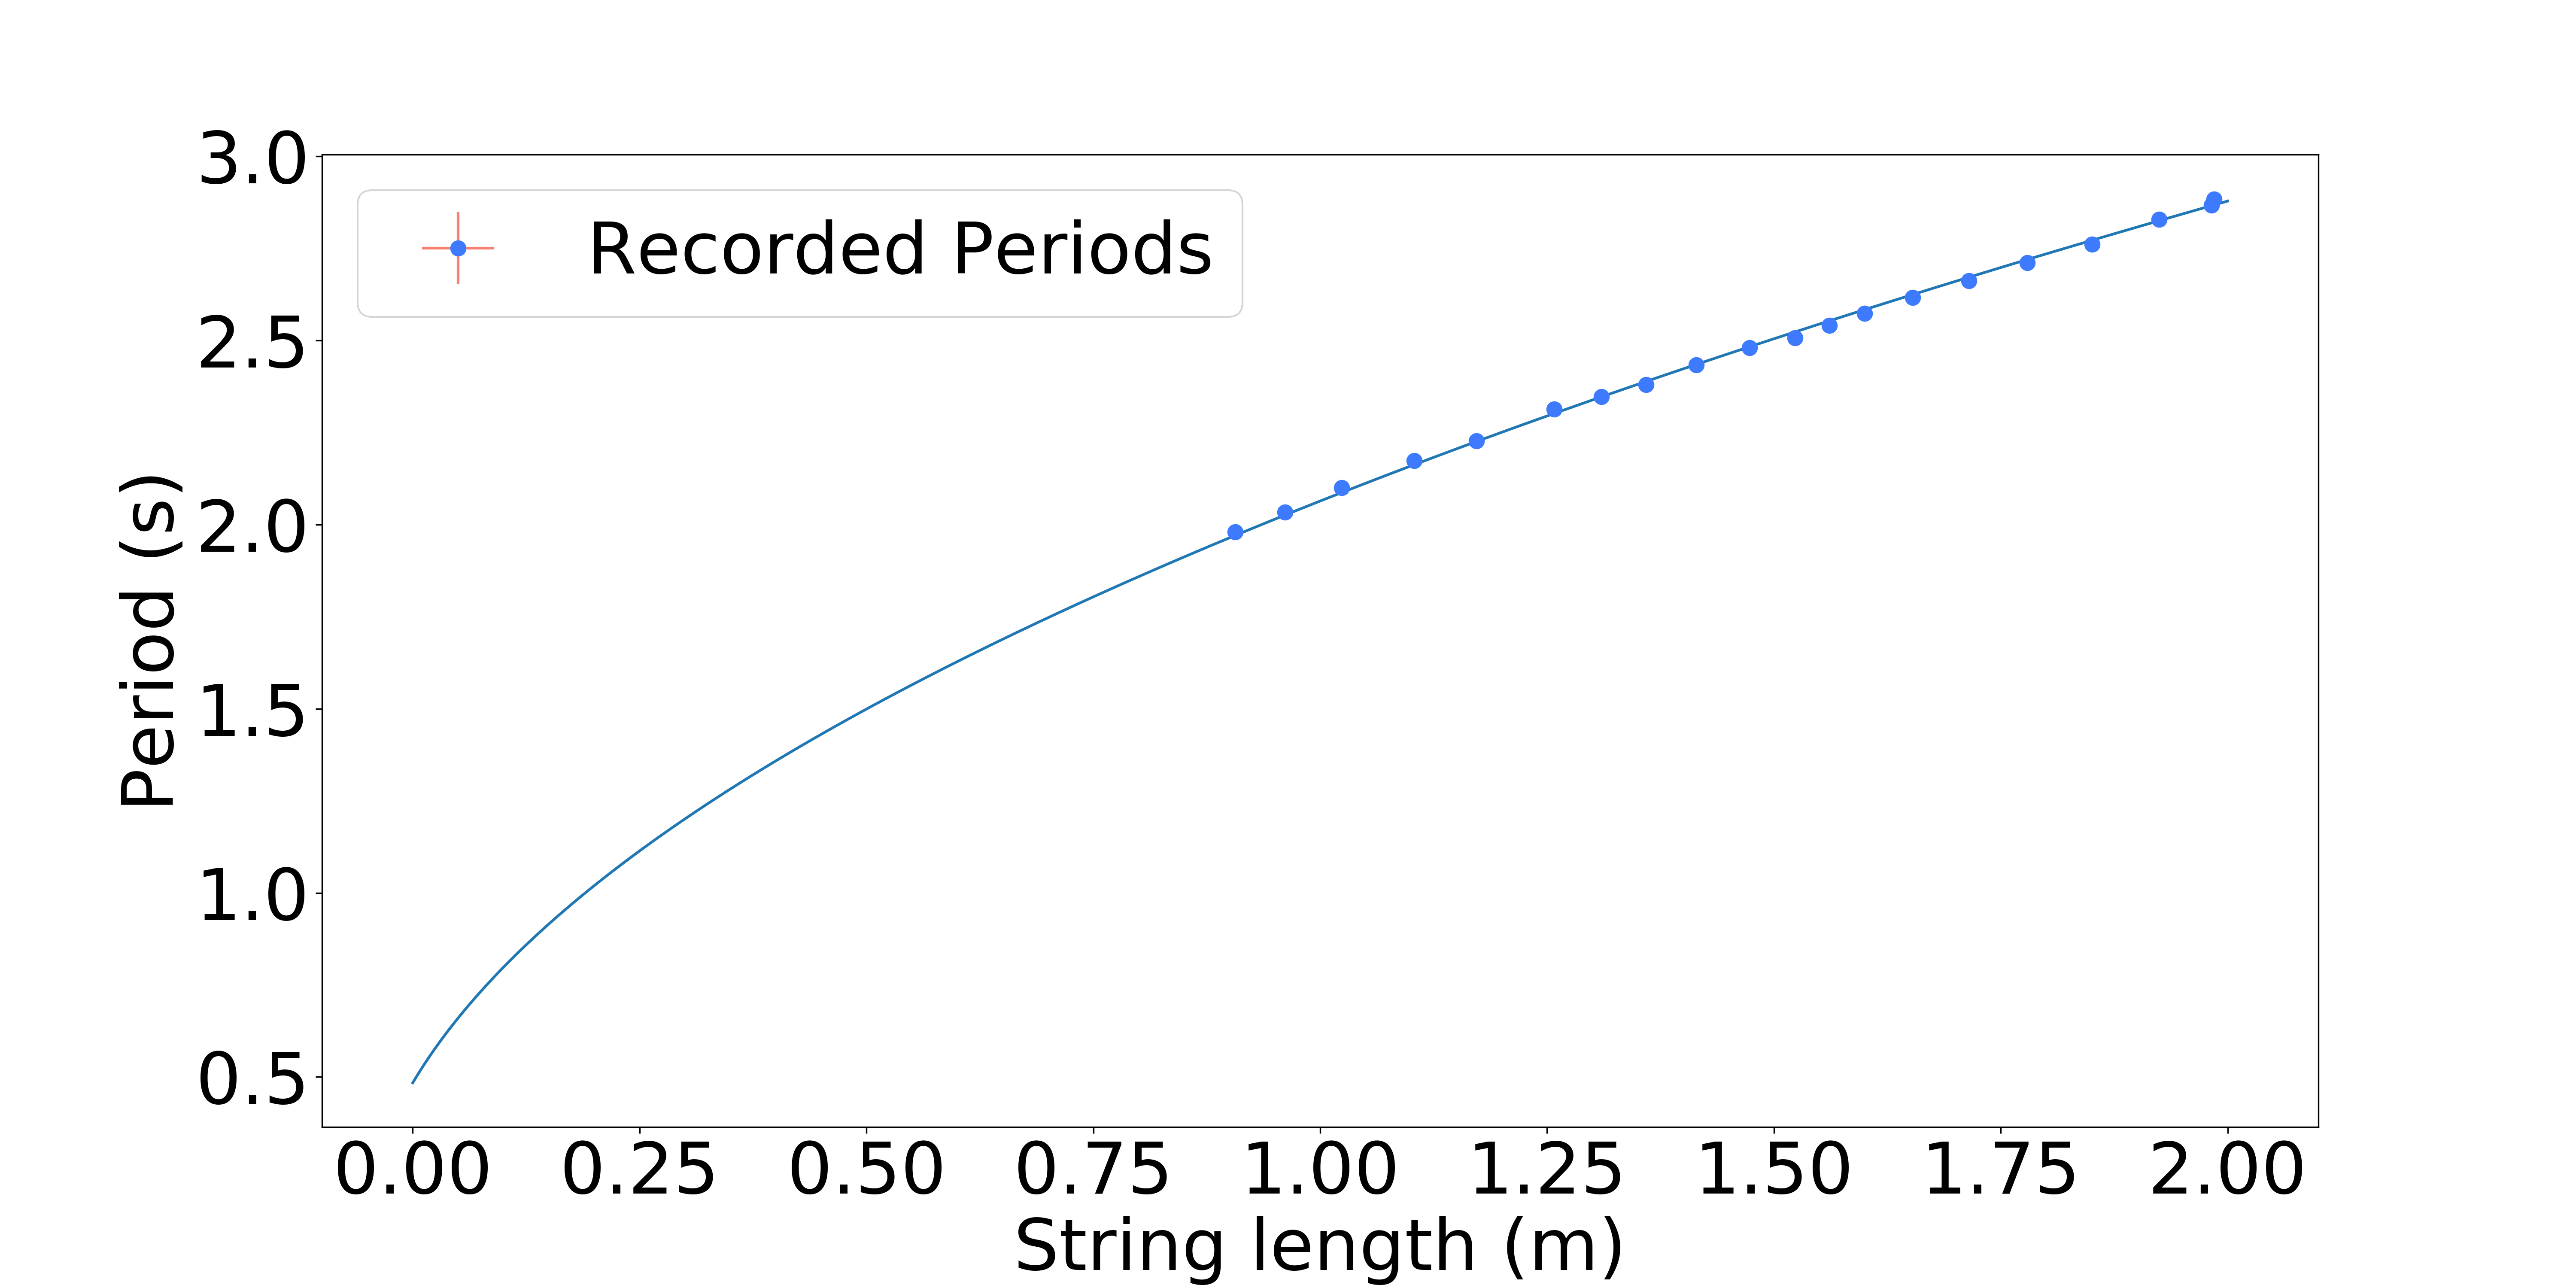
\includegraphics[width=\linewidth]{Figures/normal_2.png}

    \caption{A plot of the period against the length of the string, both linearized (above) and the original (below). Only half the data points were graphed this time to keep the string length high.}
    \label{fig:plot-2}
\end{figure}
This linearization has a slope and intercept of:
\begin{align}
    m &= 3.97 \pm 0.03 \si{\second\squared\per\meter} \\ 
    b &= 0.31 \pm 0.04 \si{\second\squared}
    \label{eq:}
\end{align}
By only looking at trials where a long string was used, the data agrees with the theoretical prediction:
\begin{equation}
    T^2 = \frac{4\pi^2}{g}\left(\ell+\Delta L\right)
    \label{eq:}
\end{equation}
where the theoretical slope is
\begin{equation}
    m_\text{theory} = \frac{4\pi^2}{9.8\pm 0.05} = 4.03 \pm 0.02 \si{\second\squared\per\meter}.
    \label{eq:mtheory}
\end{equation}
This means that the distance from the end of the string to the center of mass is:
\begin{equation}
    \Delta \ell = 0.08 \pm 0.01\si{\meter} 
    \label{eq:}
\end{equation}
We can use this information to make sense of the original value for the slope if we were to look at all data. From equation \ref{eq:proper}, we have:
\begin{equation}
    T^2 = \frac{4\pi^2}{g}\ell \left(1+\frac{\beta d^2}{\ell^2}\right)
\end{equation}
Here, the slope would be dependent on $\ell$, but since the additional factor is greater than one, the slope would always be greater than $\frac{4\pi^2}{g}$, which explains a higher overall slope when the entire data is fitted. We can provide a lower bound for $\beta$ by considering the minimum length $\ell=0.25\si{\meter}$. Since the length of the bottle is $d=0.145 \pm 0.001 \si{\meter}$, we have:
\begin{equation}
    \beta = \frac{0.25^2}{d^2} \cdot \frac{4.16 \pm 0.02}{\left(\frac{4\pi^2}{g}\right)}-1 = 0.09 \pm 0.02
    \label{eq:}
\end{equation}
This is roughly on the order of magnitude of $\beta$ for a uniform cylinder, which is $\beta=\frac{1}{12}$, so the model for small lengths can be considered relatively reasonable. To verify that the power law is $n=\frac{1}{2}$, we can plot the logarithm of the length to the center of mass $\log(\ell_\text{cm})$ with respect to the logarithm of the period $\log(T)$. Therefore, if the relationship between the two were $T = (C\ell_\text{cm})^n$, then the log-log plot would yield
\begin{equation}
    \log(T) = n\left(\log(\ell_\text{cm}) + \log(C)\right)
    \label{eq:}
\end{equation}
giving $n$ as the slope and $n\log(C)$ as the y-intercept. This is shown in figure \ref{fig:log-2}.
\begin{figure}[!h]
    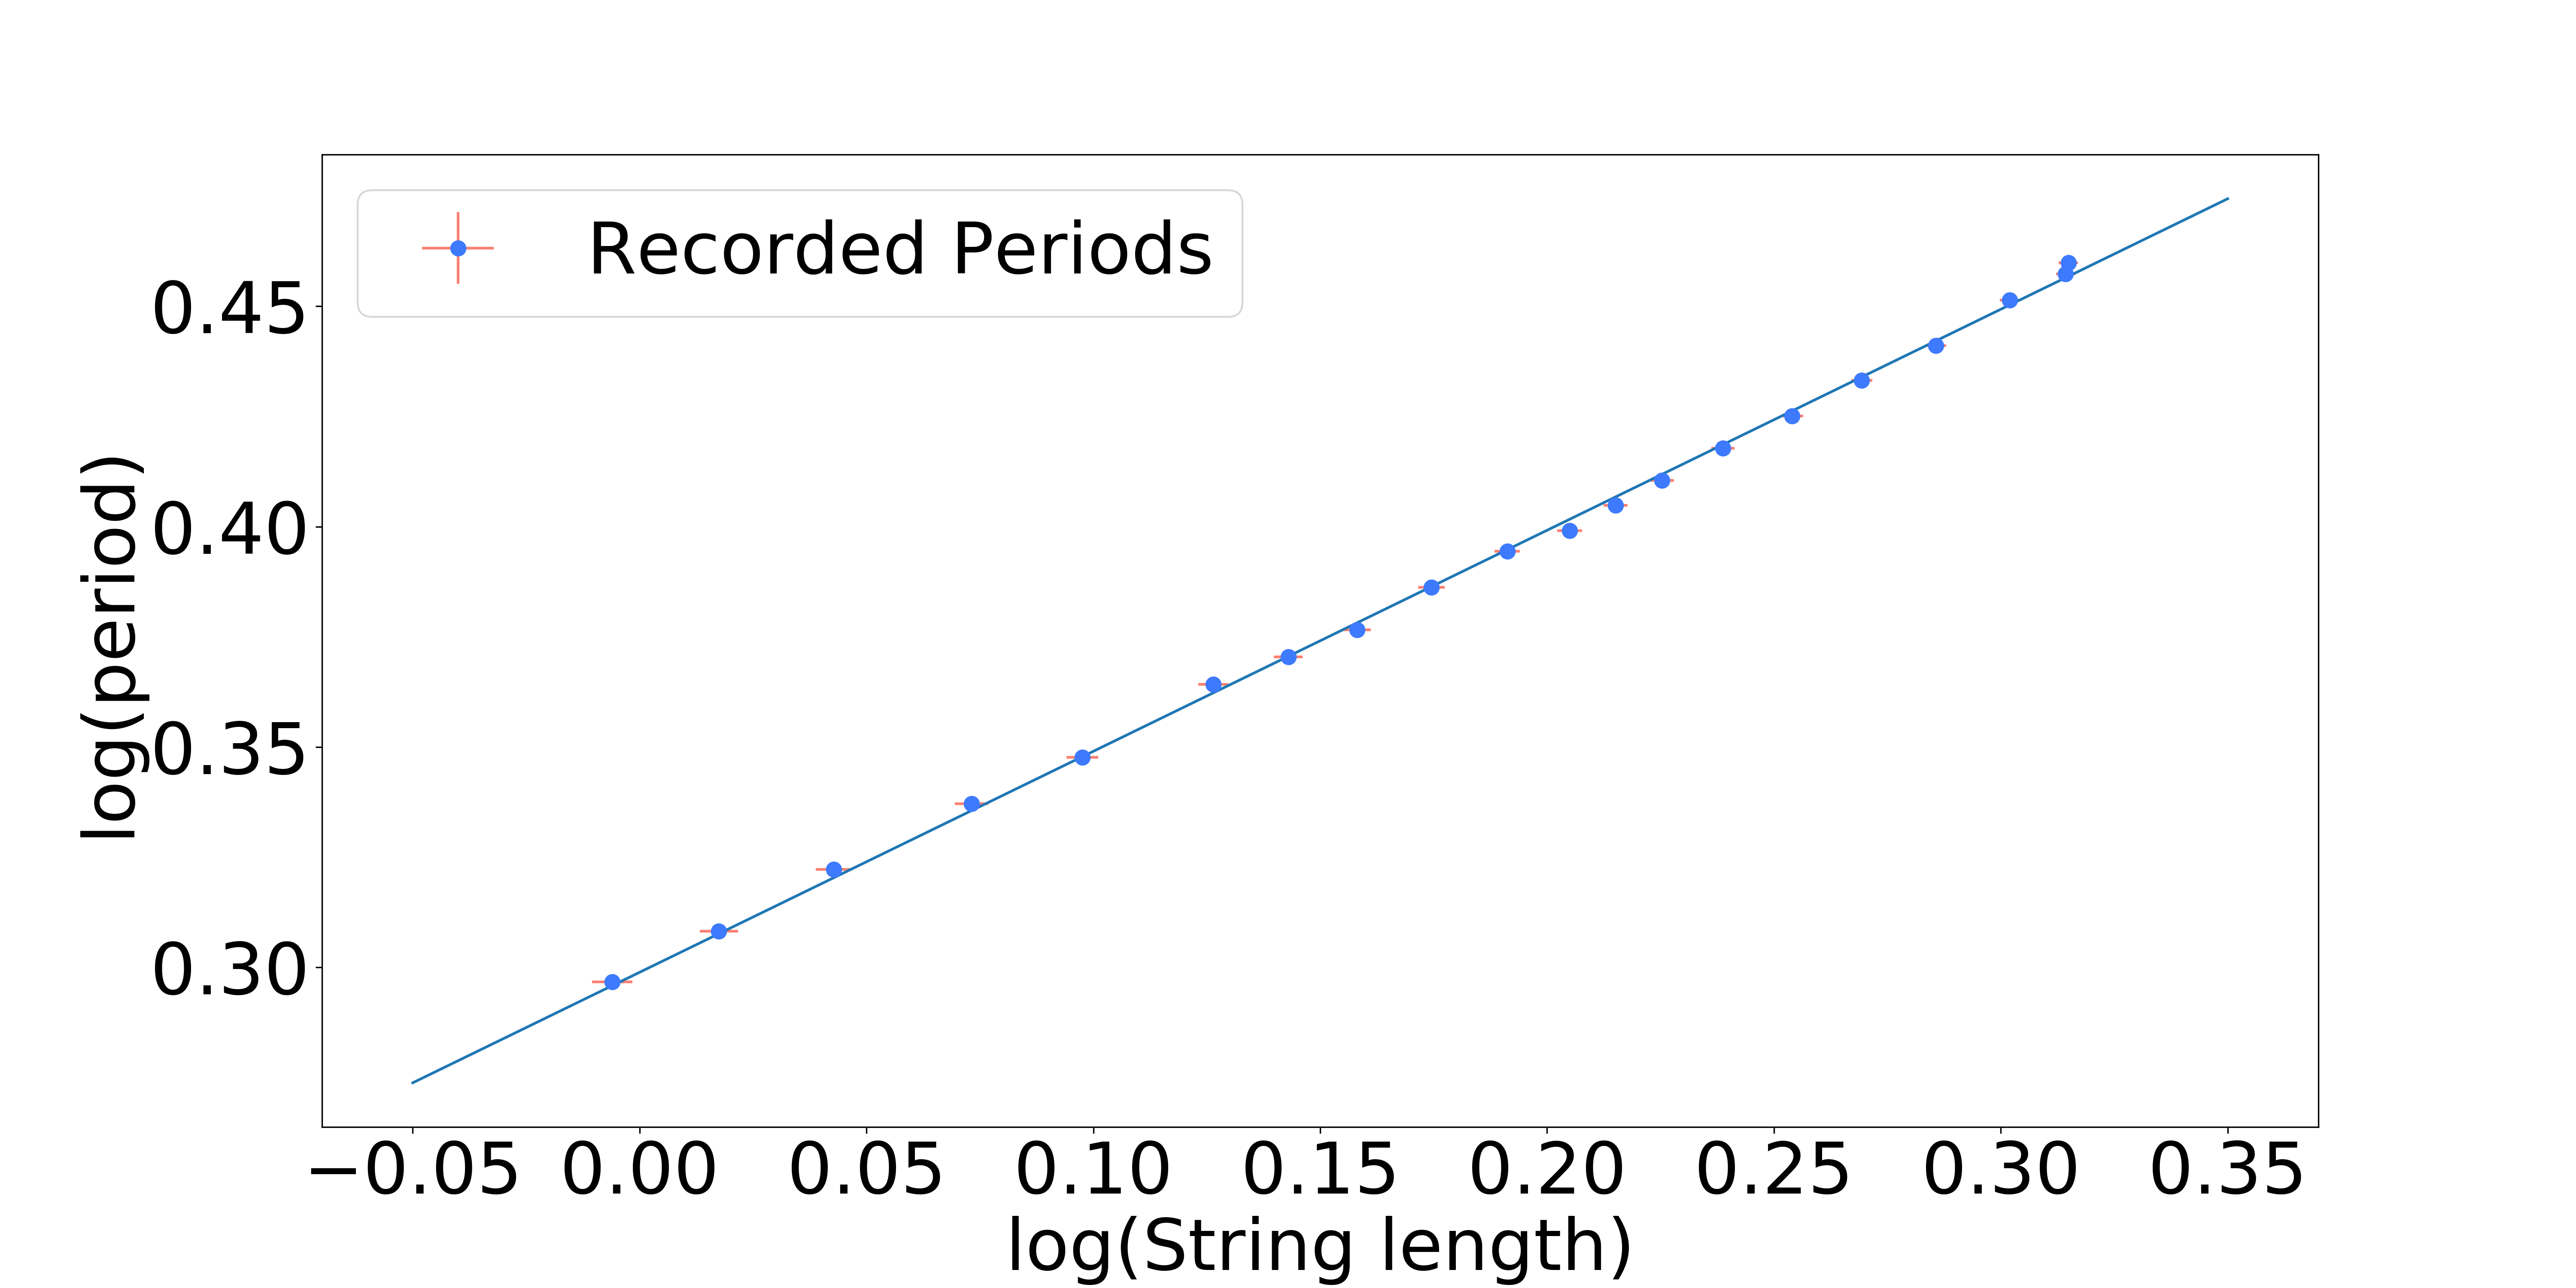
\includegraphics[width=\linewidth]{Figures/log_2.png}

    \caption{A log log plot of the period vs the distance to the center of mass, which was calculated from the previous analysis. Note that only half of the data with large values for length were plotted, in order to ensure that other effects were not important.}
    \label{fig:log-2}
\end{figure}
The slope $m$ and the y-intercept $b$ are:
\begin{align}
    m &= 0.501 \pm 0.004 \\ 
    b &= 0.2989 \pm 0.0009
\end{align}
Here, all units are scaled in such a way that they are dimensionless. Since the power is given by the slope, it agrees with the theoretical model where the relationship between period and length was a square root function. We can also verify that the theoretically predicted $y$ intercept is:
\begin{equation}
    b_\text{theory} = \frac{1}{2}\log\left(\frac{4\pi^2}{g}\right) = 0.303 \pm 0.001
    \label{eq:}
\end{equation}
which roughly agrees with the value obtained from the logarithmic plot.
\subsection{Mass Dependance}
Various masses from $0.029\si{\kilogram}$ to $0.338\si{\kilogram}$ were used for the pendulum, and shown in figure \ref{fig:mass-simple}.
\begin{figure}[!h]
    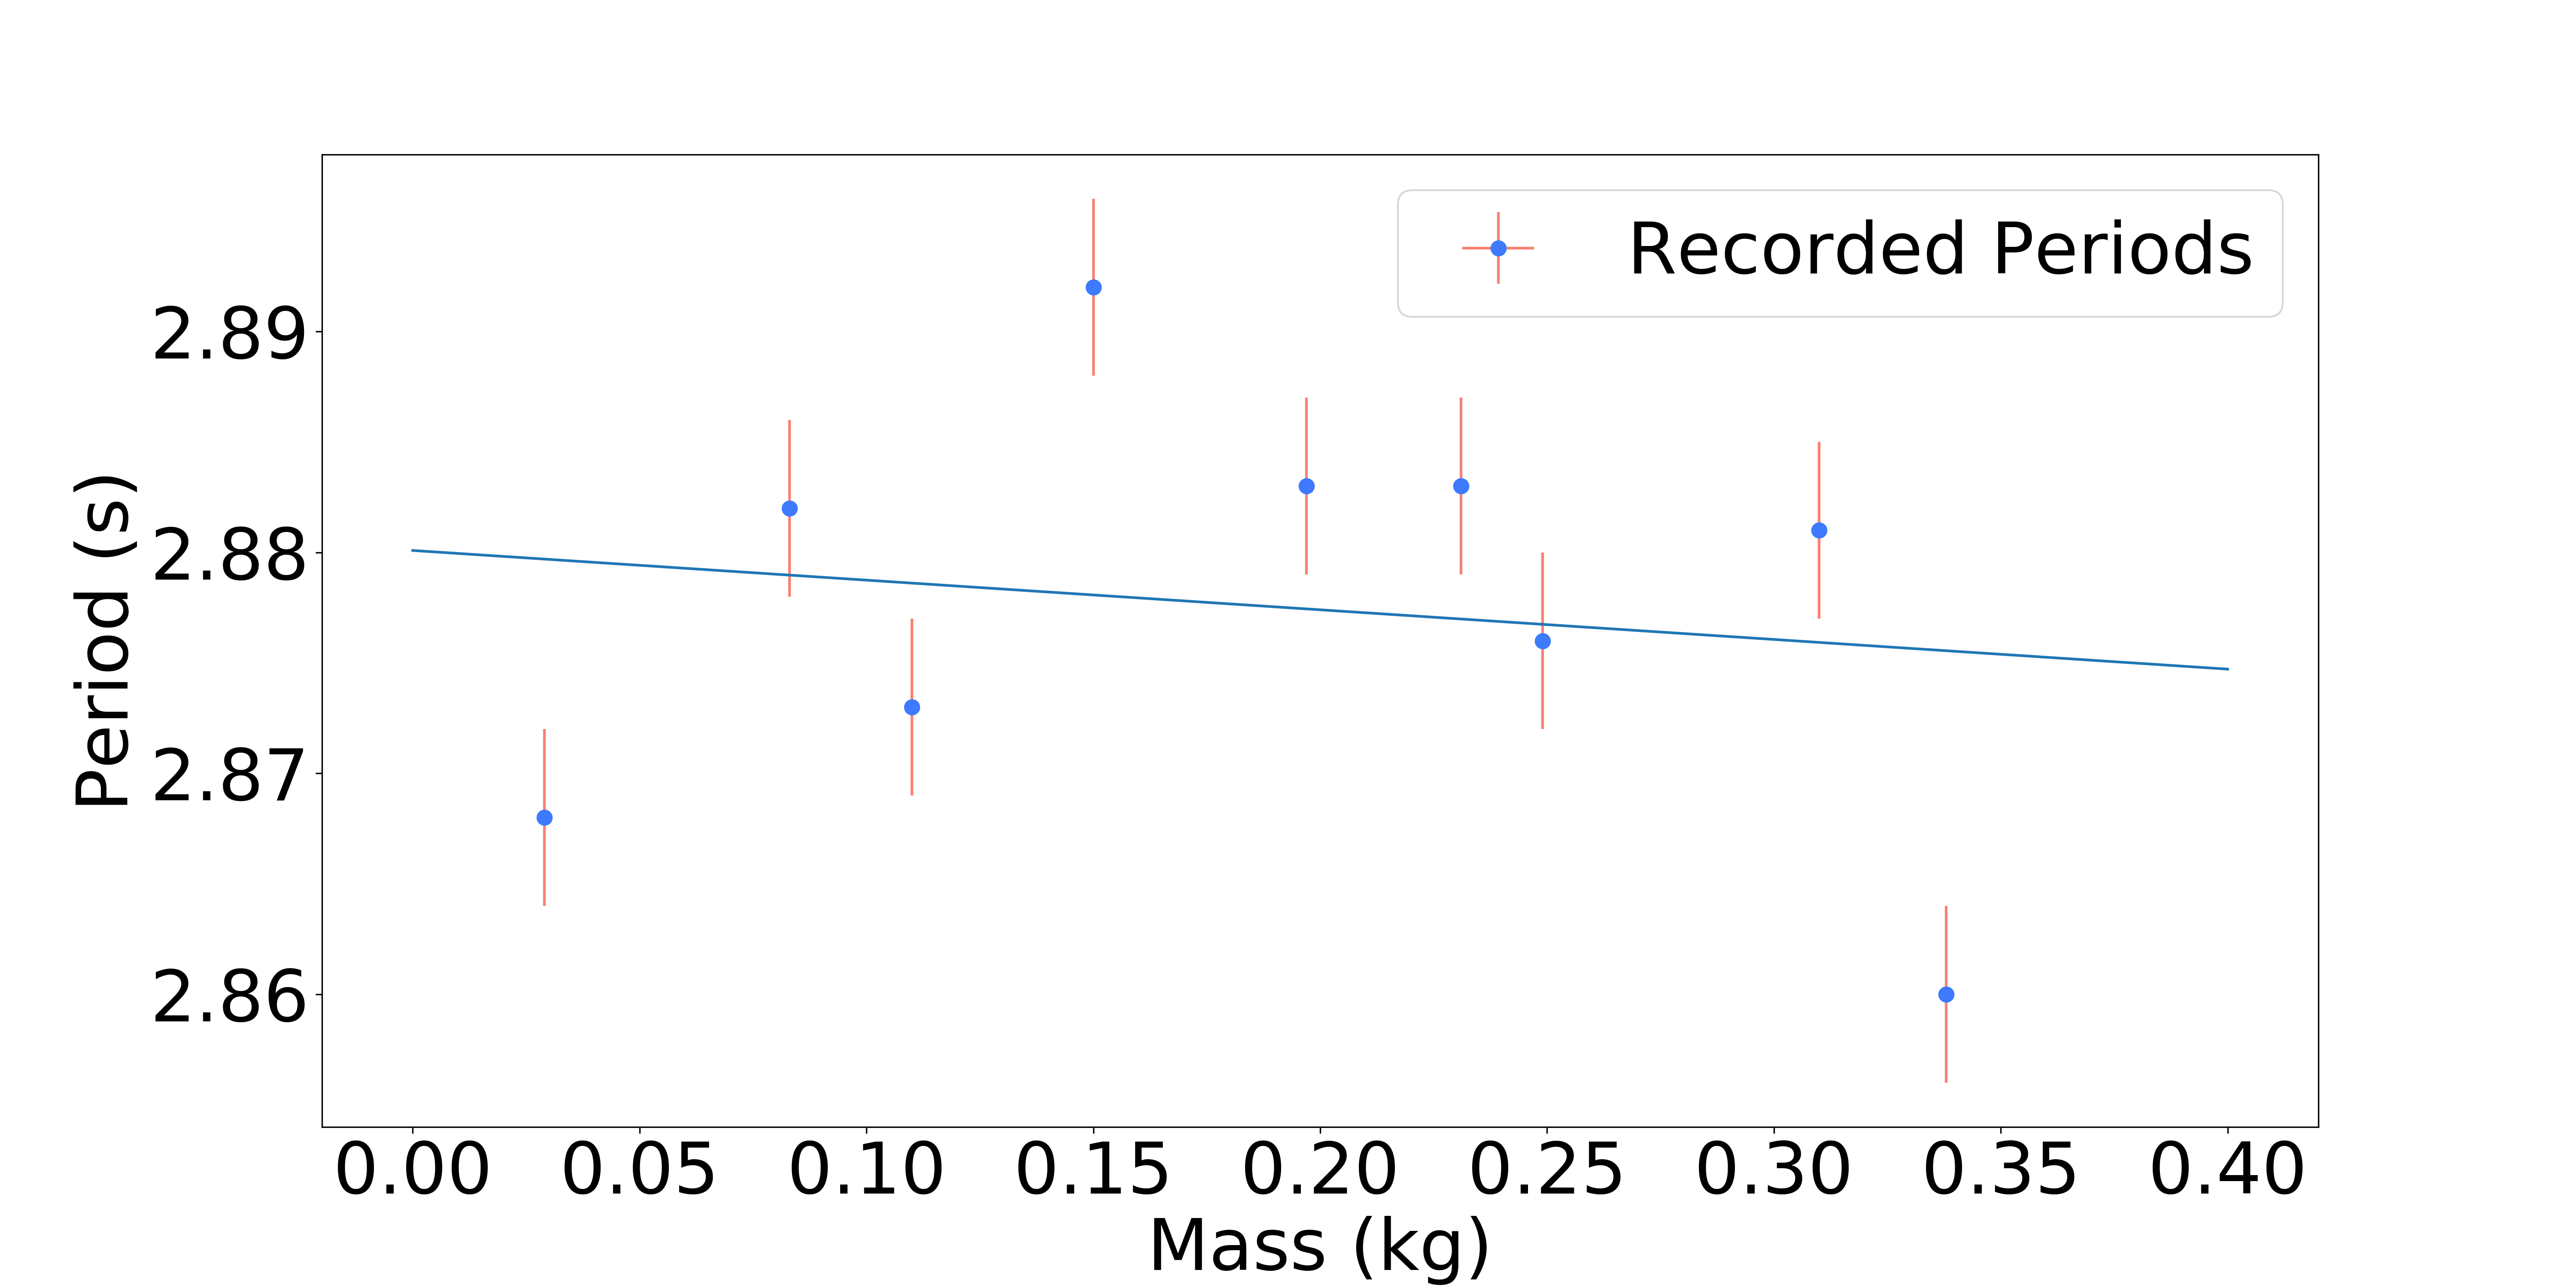
\includegraphics[width=\linewidth]{Figures/mass_simple.png}

    \caption{A plot of the period against the mass of the pendulum. Notice that the variations are similar in size to the uncertainties.}
    \label{fig:mass-simple}
\end{figure}
If a linear fit is used, the slope is given by:
\begin{equation}
    m = -0.01 \pm 0.03
    \label{eq:}
\end{equation}
which is effectively zero. As mentioned in the introduction, the instrumentation is insensitive enough that any variation in the center of mass due to changing the water level will not be noticeable, so this behaviour is expected.
\section{Discussion}
\subsection{Length Dependance}
The precision of all measurements were extremely high. Since there were over $200$ data points, but they were merged together in groups of five, the time uncertainty for the period will be negligible. The length measurements were done by a computer, and ideally, they should be overestimated the same amount of times they are underestimated such that the average length is very precise as well. This is why error bars were barely noticeable. However, even though the experimental results seem to agree with the theoretical predictions, they were still off by a little bit. For example, the predicted slope in figure \ref{fig:plot-2} had a minimum of $4.01\si{\second\squared\per\meter}$ while the value for the experimental slope had a maximum value of $4.00\si{\second\squared\per\meter}$. These small dispecrancies are still worthy of investigation, and can be caused by two main things:
\begin{itemize}
    \item Systematic error: While measurements were very precise, they could all be consistently off the true value by some fixed amount.
    \item Incorrect model: The model introduced in the hypothesis may not be entirely correct and there can be external factors that have a larger impact than previously thought.
\end{itemize}
\subsubsection{Systematic Errors}
The largest form of systematic error would be the measurement of the length of the pendulum. However, if the length of the string was consistently measured to be smaller than the true value by a certain amount $x$, then the distance from the endpoint of the string to the center of mass of the bottle would be larger by the same amount $x$ such that $\ell_\text{cm}$ is a constant. Furthermore, shifting the length by a fixed amount does not affect the value of the slope, only the $y$ intercept.

Another way the string could be measured incorrectly is an incorrect scaling factor to convert from pixels to meters. While a ruler was placed in the background to set a scale, that scale was found to be inaccurate and only served to ensure the final numbers were in the right order of magnitude. An additional scaling factor was manually determined by measuring the initial $1.985\si{\meter}$ string to $\pm 0.003\si{\centi\meter}$ accuracy. This fairly large uncertainty comes from the fact that multiple measurements had to be made and the string was attached at an angle such that the vertical distance the string extends is not equal to the length of the string. This means that the length of the string could be scaled up or scaled down by a factor of 
\begin{equation}
    \frac{\ell_\text{measured}}{\ell_\text{true}} = \left(1 \pm \frac{0.003}{1.98}\right)
    \label{eq:}
\end{equation}
This means that if the slope is $m$, then it adds on another uncertainty of around:
\begin{equation}
    \delta m = m\left(\frac{0.003}{1.98}\right) \approx 0.01 \si{\second\squared\per\meter}
    \label{eq:}
\end{equation}
which is approximately the difference between the upper and lower bounds of the theoretical value and the experimental value for the slope of the linearized graph.
\subsubsection{Other Factors}
Contradictions appear to arise when the original function is fit to the function:
\begin{equation}
    T = \sqrt{\alpha \cdot \frac{I+\ell_\text{cm}^2}{\ell_\text{cm}}}
    \label{eq:moment of inertia}
\end{equation}
to determine the value of $I$, which is the specific moment of inertia. This is done in \ref{fig:normal-complex}.
\begin{figure}[!h]
    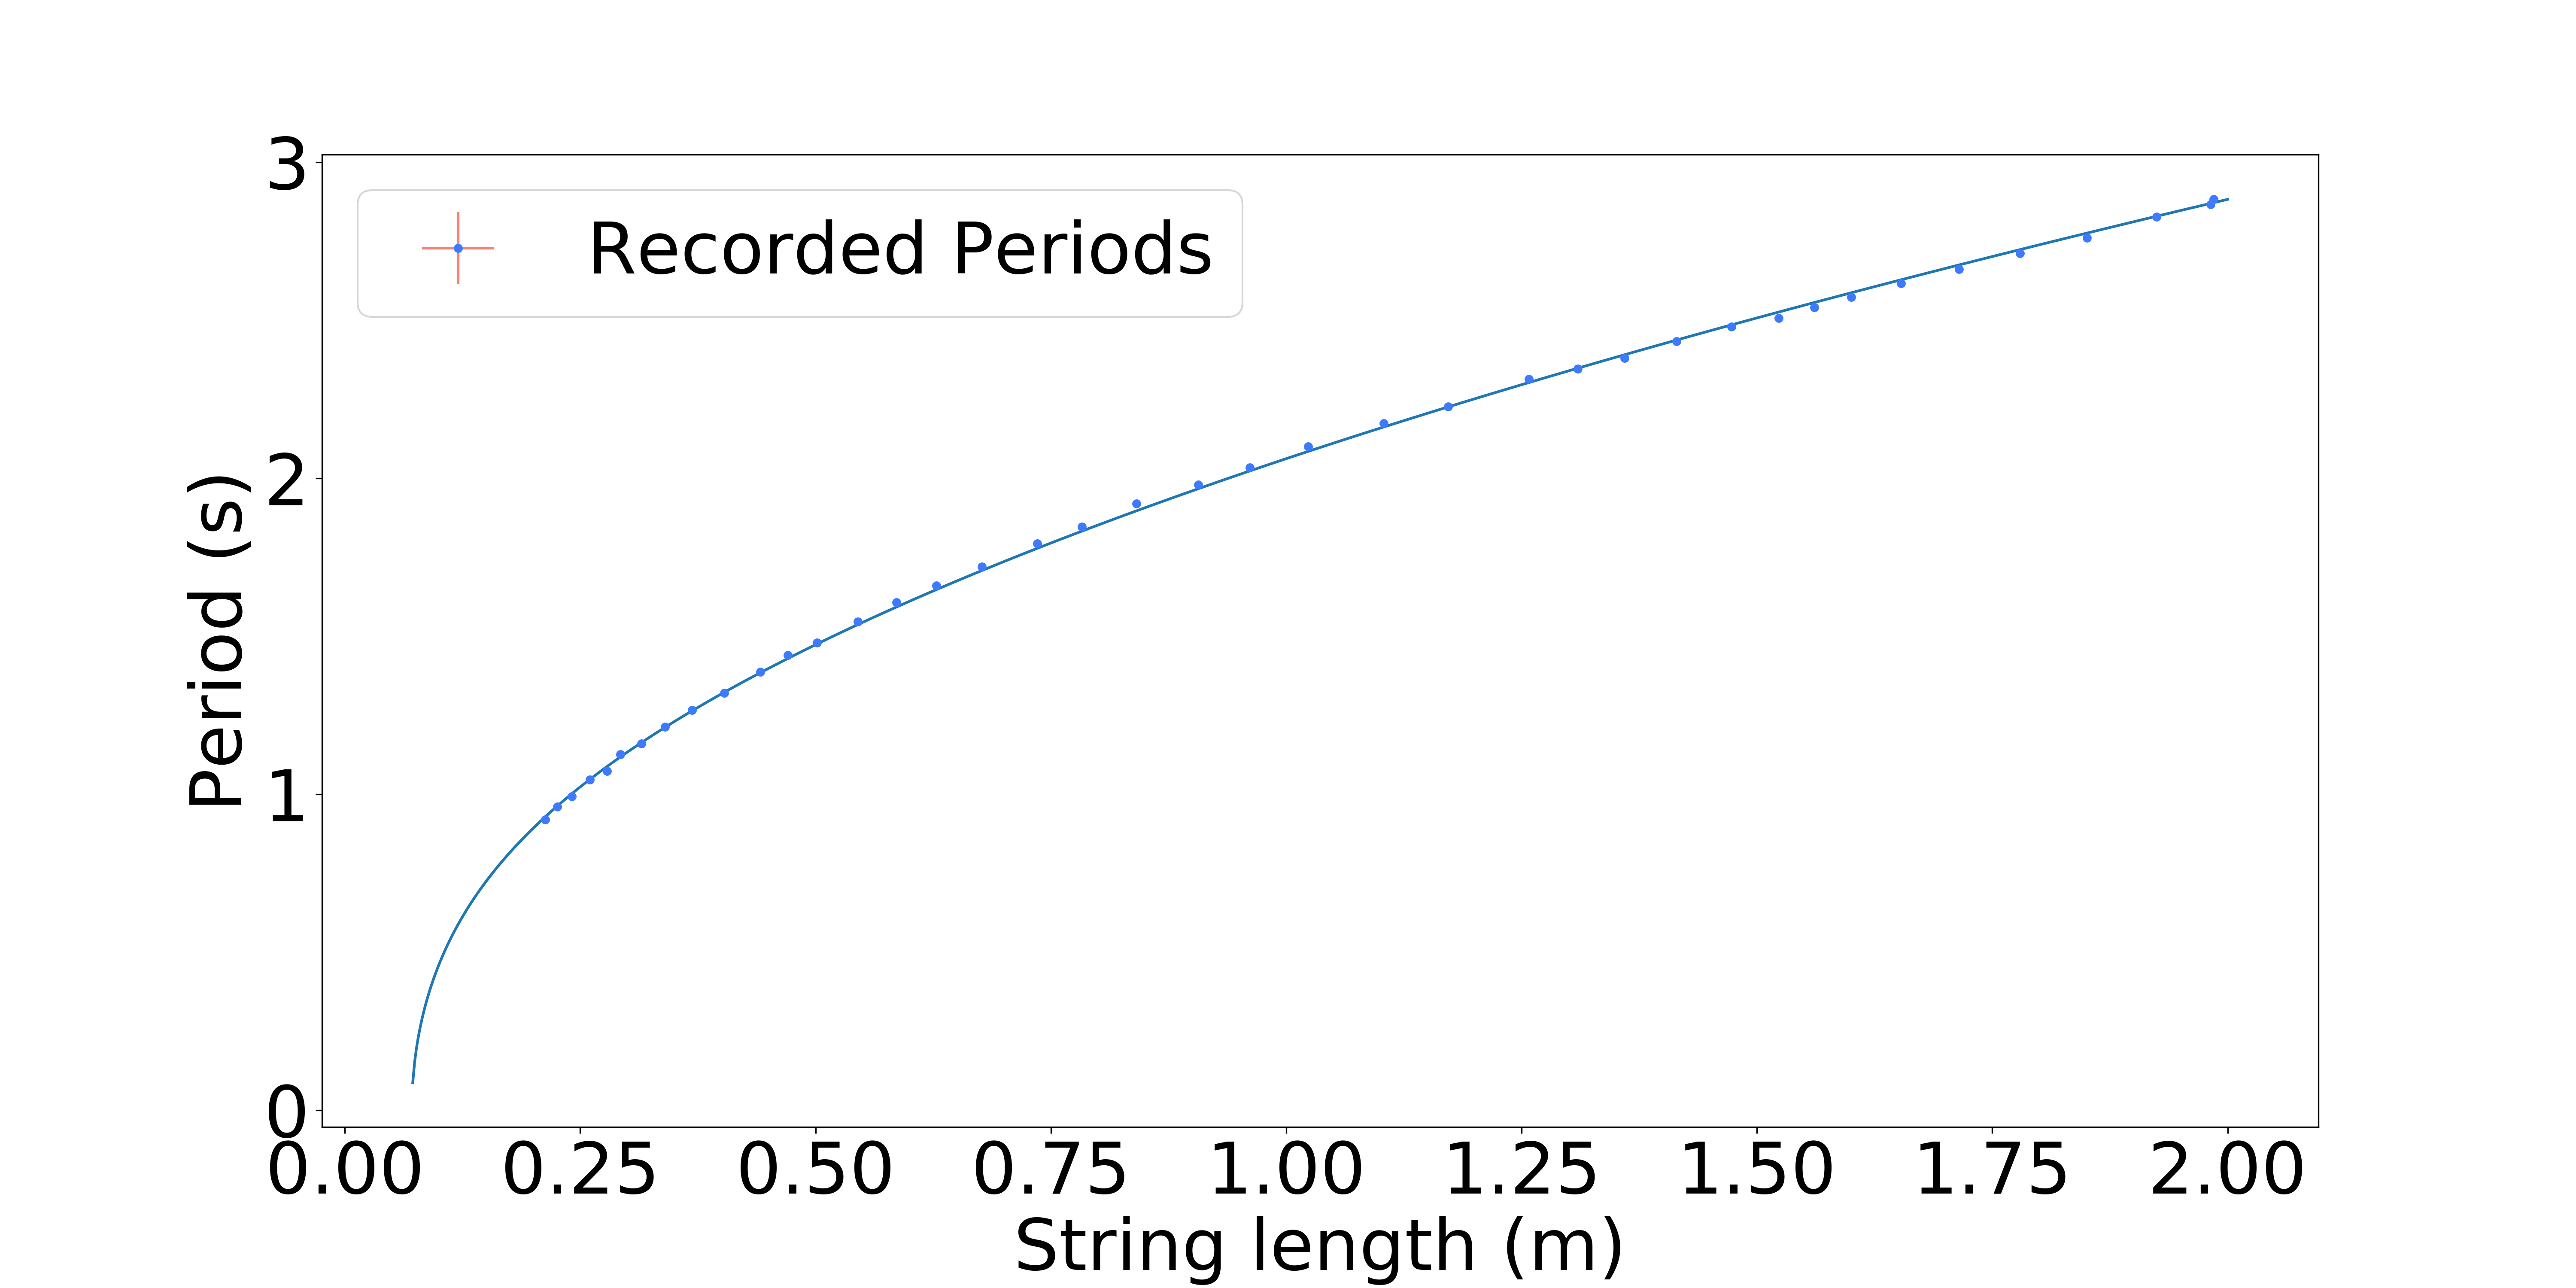
\includegraphics[width=\linewidth]{Figures/normal_complex.png}

    \caption{A plot of the period against the length of the center of mass of the pendulum. Notice that the plot visually looks much more accurate than that of \ref{fig:linear-1}.}
    \label{fig:normal-complex}
\end{figure}
The value for $\alpha$ and $I$ are given as:
\begin{align}
    \alpha &= 4.015 \pm 0.008 \si{\second\squared\per\meter}\\ 
    I &= -0.0228 \pm 0.0007 \si{\meter\squared}
\end{align}
Note that the theoretical value of $\alpha$ is given in equation \ref{eq:mtheory} as $\alpha_\text{theory}=4.03 \pm 0.02 \si{\second\squared\per\meter}$. Here, the experimental value is closer to the theoretical model than that shown in figure \ref{fig:plot-2}. However, the moment of inertia takes on a negative value, which is simply impossible! The uncertainty is also very low, so this suggests that there is something wrong with the physical model. I claim that this is due to neglecting the effects of air resistance. As shown in the first lab, the true angular frequency of an underdampened pendulum is:
\begin{equation}
    \omega = \sqrt{\omega_0^2\left(1-\left(\frac{2}{Q}\right)^2\right)}
    \label{eq:omegalol}
\end{equation}
However, both air resistance and an extra moment of inertia will tend to increase the period, not decrease it. Therefore, there is some mechanism that is adding in energy. One possible mechanism that can accomplish this is that the manual rising of the string could be increasing the angular speed. I will investigate how large of an effect this is by writing out the rotational equation of motion as:
\begin{equation}
    \frac{dL}{dt} = \frac{d}{dt}\left(m \ell^2 \omega\right) = -mg\ell\sin\theta
    \label{eq:}
\end{equation}
Applying the product rule, this gives:
\begin{align}
    2m\ell\omega \frac{d\ell}{dt} + \frac{d\omega}{dt}m\ell^2 &= -mg\ell\sin\theta \\ 
    \frac{d^2\theta}{dt^2} &= -\frac{g}{\ell}\theta + \frac{2\dot{\ell}}{\ell}\dot{\theta}
    \label{eq:}
\end{align}
The average value for $\dot{\ell}$ is $\dot{\ell}_\text{avg}=0.00440 \pm 0.00001 \si{\meter\per\second}$. The effective damping coefficient is now negative, which means that the period should be shorter than expected. Similar to \ref{eq:omegalol}, we can derive the period as:
\begin{equation}
    T = T_0\sqrt{\left(1-\frac{1}{\omega_0^2}\left(\frac{\dot{\ell}}{\ell}\right)^2\right)}
    \label{eq:}
\end{equation}
Comparing this to equation \ref{eq:moment of inertia}, which can be written as:
\begin{equation}
    T = T_0\sqrt{\left(1+\frac{I}{\ell^2}\right)}
    \label{eq:}
\end{equation}
We can derive the specific moment of inertia to then be:
\begin{equation}
    I = -\frac{\ell \dot{\ell}^2}{g} \approx -5 \times 10^{-6} \si{\meter\squared}
    \label{eq:}
\end{equation}
which is essentially negligible. It appears that there is no straightforward explanation to why the theoretical model overestimates the period. Accounting for a nonzero moment of inertia and air resistance damping effects only leads to an increase in the period, not a decrease. More experimentation needs to be done to pin down the reason behind this dispecrancy. As a result, it is likely this is due to a systematic error of how certain measurements were made, that were not included in the previous section. For example, perhaps I have overestimated the precision at which the string length can be measured. It is recommended that the experiment be completed again, including any or a combination of the following modifications:
\begin{itemize}
    \item Using a small but heavy mass.
    \item Taking period measurements in multiple independent methods.
    \item Changing the string length in a different way.
    \item Measuring the string length in multiple independent methods.
\end{itemize}
\subsection{Mass Dependance}
\subsubsection{Systematic Errors}
Many systematic errors that appear in the length dependance are not significant when looking at the length dependance. As long as the length of the string can be measured precisely, it does not matter how accurately it is measured. For example, it is perfectly acceptable even if every measurement of the length is larger than the true amount by $5\si{\centi\meter}$, as long as this error is consistent. This is because I am looking if there is a trend when the mass is changed.

A kitchen scale was used to measure the mass of the bottle, which has a precision of $\pm 0.5\si{\gram}$. Timing was done with a stopwatch and from the mini experiment described in the Introduction, I found myself to stop the stopwatch earlier roughly the same amount of times I stopped it late. As a result, it is very unlikely that there are any systematic errors that could affect the measurements.

\subsubsection{Other Factors}
The center of mass of the system can change, but this is already analyzed in the Introduction, which showed that variations in period due to this is very likely unnoticeable. Another contributing factor could be air resistance. From equation \ref{eq:omegalol}, we can show that the period of the pendulum is:
\begin{equation}
    T = T_0\sqrt{1+\left(\frac{2}{Q}\right)^2}
    \label{eq:}
\end{equation}
Since $Q \equiv \frac{m}{b}\sqrt{\frac{\ell}{g}}$, decreasing the mass effectively decreases the $Q$ factor by the same proportion. The pendulum used has an average center of mass of $\ell_\text{cm}=2.015 \pm 0.003 \si{\meter}$, so the $Q$ factor is around:
\begin{equation}
    Q_\text{new} = Q_\text{before}\sqrt{\frac{201.5}{115}} = 433 \pm 4
    \label{eq:}
\end{equation}
where the quality factor at a length of $\ell_\text{cm}=115\si{\centi\meter}$ was $Q_\text{before}=247 \pm 2$. This means that for a mass $m$, the quality factor is:
\begin{equation}
    Q = \frac{m}{338} \cdot \left(443 \pm 4\right)
    \label{eq:}
\end{equation}
For the lowest mass, this gives a $Q$ factor of approximately:
\begin{equation}
    Q = 37.1 \pm 0.3
    \label{eq:}
\end{equation}
This means that the relative error in the period uncertainty is around:
\begin{equation}
    \delta T = T\left(\frac{2}{Q^2}\right) = 0.004
    \label{eq:}
\end{equation}
which also coincidentally happened to be within my measurement error. Therefore, the mass does not greatly impact the motion of the pendulum. The fluctuations could very easily be caused by external factors such as a changing center of mass and air resistance. The next steps would be to develop a method to lower measurement uncertainties such that these other factors can be quantified, measured, and accounted for. One possible method is to poke a small hole such that water slowly drains out. However, I will need to be careful as large holes will cause the water to drain out too quickly and small holes will cause surface tension to have a large effect.
\section{Conclusion}
In conclusion, the experiment supported the validity of the approximation $T=2\pi\sqrt{\frac{\ell_\text{cm}}{g}}$ as the period of a pendulum. Both the length and the mass affected the period how it was expected to. However, when accounting for other effects such as air resistance, a changing center of mass, and a nonzero moment of inertia, the proposed models to account for these effects do not hold up well to the experiment. They reveal inconsistencies between theory and experiment.

It is strongly recommended that this experiment be completed again. For verifying the length dependance, a heavy small object should replace the water bottle and for the mass dependance, a small hole should be poked to allow water to leak out, which slowly decreases the mass. For both experiments, length and time measurements should be made to even higher accuracy and precision in order to quantify the additional effects listed above.

\appendix
\section{Data}
As always, the data points, as well as the Python code is provided on \href{https://github.com/QiLinXue/pendulum-labs/}{Github}, for accountability purposes.
\end{document}